\chapter{Хэрэгжүүлэлт}
\section{Сонгосон технологи}
\subsection{Nextjs \& Reactjs}
\subsubsection{Declarative}
React нь хэрэглэгчийн интерактив интерфейс бүтээхийг хялбарчилдаг. Aппликейшны state бүрд зориулсан энгийн бүтэц зохион байгуулахаас гадна, React нь өгөгдөл өөрчлөгдөхөд яг зөв компонентоо өөрчлөн рендер хийдэг. Declarative бүтэц нь кодыг тань debug хийхэд хялбар болгохоос гадна, ажиллагаа нь илүү тодорхой болдог

\subsubsection{Компонент-д тулгуурласан}
Бие даан state-ээ удирддаг маш энгийн компонент бичиж, эдгээрийг хольж найруулан нарийн бүтэцтэй хэрэглэгчийн интерфейс бүтээ.

Компонентийн логик нь тэмплэйт-ээр бус JavaScript-ээр бичигддэг учраас өгөгдлийг апп хооронд хялбар дамжуулж, DOM-оос state-ээ тусд нь байлгаж чадна.

\subsubsection{Nextjs}
Netflix, TikTok, Hulu, Twitch, Nike гэсэн орчин үеийн аваргууд ашигладаг энэхүү орчин үеийн фрэймворк нь React технологи дээр үндэслэгдсэн бөгөөд Frontend Backend хоёр талд хоёуланд нь ажилладаг веб аппуудыг хийх чадвартайгаараа бусдаасаа давуу юм. Next.js -ийн үндсэн дизайн нь клиент болон сервер талын аль алиных давуу талыг ашиглаж чаддаг, ямар нэг дутагдалгүй веб сайтыг яаж хамгийн хурдан хялбар бүтээх вэ гэдгийг бодож тусгасан байдаг. Next.js нь сервер талд react компонентуудыг рендерлэн энгийн html, css, json файл болгон хувиргах замаар ажилладаг бөгөөд 2020 оноос олон нийтэд танигдсан JAMStack технологи болон статик сайт, автоматаар статик хуудас үүсгэх, CDN deployment, сервергүй функц, тэг тохиргоо, файлын системийн рүүтинг (PHP-ээс санаа авсан), SWR (stale while revalidate), сервер талд рендерлэх зэрэг асар олон орчин үеийн шинэхэн технологиудыг бүгдийг хийж чаддаг анхны бүрэн веб фрэймворк гэж хэлж болно.\cite{Reactjs}
\subsection{tRPC (Back End)}

Энгийнээр хэлбэл, tRPC нь клиент болон сервер хоорондоо сүлжээгээр харилцаж болох API (Application Programming Interfaces) бүтээх хэрэгсэл юм. Энэ нь хувьсагчийн төрлүүдийг нягт зааж өгч Front-End Back-End хоёрийг холбож ажилладаг. Жишээ нь хэрвээ сервер тал дээр ажиллаж байгаа хөгжүүлэгч, функцын параметр солиход энгийн REST api эсвэл Graphql түүнийг мэдэж чадахгүй юм. Харин tRPC нь шууд алдаа болж харагдах ба хөгжүүлэлтийн орчинд Back-end Front-end хоёр холбогдож ажилдаг гэдгээрээ давуу юм. Ингэснээр хөгжүүлэхэд илүү хялбар, инжинерт илүү ээлтэй болдог билээ.
Кодыг \ref{lst:docker-compose}
\subsection{AWS S3 объект агуулах}
AWS S3 (Amazon Simple Storage Service) нь Amazon Web Services (AWS) дээрх өгөгдөл, мэдээллийг онлайнаар нөөцлөх, архивлахад зориулагдсан хязгааргүй өргөтгөх боломжтой, өндөр хурдтай, вэб технологит суурилсан үүлэн хадгалах үйлчилгээ юм. Энэ нь вэбийн хаанаас ч хүссэн үедээ ямар ч хэмжээний өгөгдлийг хадгалах, сэргээхэд ашиглаж болно.
\subsection{AWS KMS}
AWS Түлхүүр Удирдлагын Үйлчилгээ (KMS) нь криптографын түлхүүрүүдийг үүсгэх, хянахад хялбар болгодог. Мөн түүнчлэн түлхүүр нь ашиглагдаагүй хадгалагдаж байх үедээ шифрлэгдсэн байдаг.
Энэхүү үйлчилгээ нь бусад AWS үйлчилгээнүүдтэй нэгтгэгдсэн тул эдгээр үйлчилгээнд хадгалсан өгөгдлийг шифрлэх, кодыг тайлах түлхүүрүүдэд хандах хандалтыг хянахад хялбар болгодог.

\subsection{Dockerizing}
Орчин үеийн нэгэн гайхалтай технологи бол контайнерчлах юм. Яагаад Docker чухал вэ гэвэл, ямар нэгэн систем хөгжүүлэгчийн компьютер аль эсвэл ямар сервер дээр ажиллаж байгаагаас үл хамааран проргам нь өөрийн тусдаа орчинд ажиллах юм. Яг л Virtual machine шиг гэхдээ давуу тал нь Docker host system-ийнхээ цөмийг (kernel)-г ашигладаг учраас маш бага хэмжээгий зай, нөөц ашигладаг.
\subsection{CI/CD}
Мөн сүүлийн үед маш их өргөн түгж байгаа ойлголт бол Continuous Integration/Continuous Deployment.
Энэ нь проргам хангамж ямар ч нөхцөлд хөгжүүлэлт тасралтгүй явж байх орчноор хангадаг ба системд хэзээ ч тасалдал үүсгэхгүй мөн хүний оролцоог маш бага байлгах давуу талтай.\footnote{Дадлагын ажлаасаа иш татав. https://github.com/b4ljk/internship-report}.

\section{Ажиллагаа}
\subsection{Гарын үсэг зурах}
\subsubsection{Сервер талд ажиллах}
\begin{enumerate}
	\item Хэрэглэгчийн оруулсан файлыг объект агуулахаас (AWS S3) татаж авах.
	\item Файлын бинари (binary) хэсгийг SHA256 алгоритм ашиглан хайш утгыг тооцоолох.
	\item Хэрэглэгчийн хувийн түлхүүрийг аюулгүй хадгалах орчноос авах (AWS KMS).
	\item Хувийн түлхүүрийг ашиглах хайш утгыг шифрлэх.
	\item Шифрлэгдсэн утгыг өгөгдлийг сан руу хадгалах.
	\item Шифрлэгдсэн утга буюу гарын үсгийг олон улсын стандартын дагуу PDF файл руу нэмэх.
	\item Шинээр үүссэн буюу шифрлэгдсэн файлыг объект агуулах руу хуулах.
	\item Нэг удаагийн татаж авах холбоосыг хэрэглэгчид өгөх.
\end{enumerate}
\subsubsection{Хэрэглэгч талд ажиллах}
\begin{enumerate}
	\item Хэрэглэгчийн өөрийн файлыг оруулах.
	\item Файлын бинари (binary) хэсгийг SHA256 алгоритм ашиглан хайш утгыг тооцоолох.
	\item Хэрэглэгч хувийн түлхүүрээ оруулах.
	\item Хувийн түлхүүрийг ашиглах хайш утгыг шифрлэх.
	\item Шифрлэгдсэн утгыг сервер рүү илгээх.
	\item Шифрлэгдсэн утга буюу гарын үсгийг олон улсын стандартын дагуу PDF файл руу нэмэх.
	\item Хэрэглэгч талд гарын үсэг зурсан файл үүсэх.
\end{enumerate}

\section{Хөгжүүлэлт}

\subsection{Хөгжүүлэлтийн орчныг бэлдэх}
Миний хувьд хөгжүүлэлтийн орчныг бэлдсэнээр нийт ажлын тал нь дуусдаг. Энэхүү судалгааны ажлын практик хэсэгт би NextJS, tRPC, PrismaORM, PlanetscaleDB, AWS зэргийг ашиглан хөгжүүлэлт хийх билээ. NextJS нь монолитик төсөл хийхэд тохиромжтой ба би төслийн сервер, клайнт талуудыг нэг repository-д хадгалж байгаа юмаа. Version Control System дээр Github-г соногосон юм. Кодын фолдер бүтэцmai нь дараах байдлаар байна.

\begin{figure}[h]
	\centering
	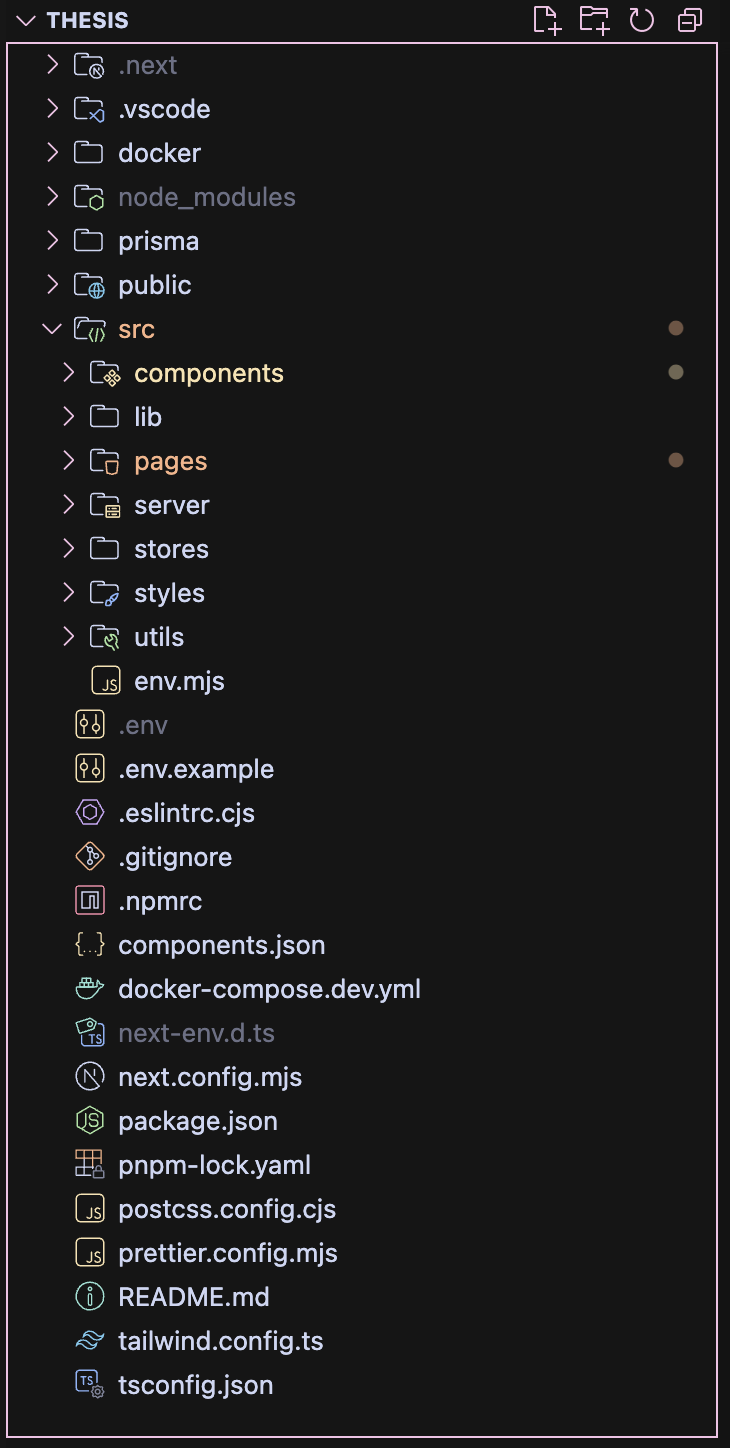
\includegraphics[scale=0.55]{assets/web/structure.png}
	\caption{Фолдерийн бүтэц}
	\label{fig:architecture}
\end{figure}
\begin{itemize}
	\item \textbf{.github/workflows} - CI/CD хийхэд шаардлагатай файлууд
	\item \textbf{components} - React компонентууд
	\item \textbf{lib} - Хэрэглэгчийн талын шаардлагатай код туслах функцууд
	\item \textbf{pages} - NextJS дээрх хуудаснууд
	\item \textbf{prisma} - Prisma ORM-ийн өгөгдлийн сангийн зохион байгуулалт
	\item \textbf{public} - Хуудаснуудын зураг, css файлууд
	\item \textbf{server} - Сервер талын код
	\item \textbf{store} - Хэрэглэгчийн талын төлвийг (state) хадгалах сан
	\item \textbf{docker} - Dockerfile, docker-compose файлууд
\end{itemize}

\subsubsection{Өгөгдлийн сангийн зохион байгуулалт}
Призма нь өгөгдлийн сан болон, код баз хоёрын хялбараар холбоход тусладаг. Үүнийг ORM гэж нэрлэдэг ба давуу тал нь, өгөгдлийг ариутгах, өгөгдлийг сангийн зохион байгуулалт түүхийг хадгалах зэрэг ажлыг инжинер хийх шаардлаггүй болох юм.
\lstinputlisting[language=Typescript,lastline=30, caption=Prisma Датабаазын модел,label=lst:prisma,frame=single]{src/code/schema.prisma}

\subsubsection{AWS}
Амазоны санал болгодог үйлчилгээнүүдийг өөртөө тохирхийг нь ашигласнаар заавал өөрийн серверийг ажлуулах шаардлаггүй болно. Мэдээж ашиглахийн тулд AWS дээрээ тохиргоонуудыг хийх ба нууцлалын мэдээллүүдээ код дундаа оруулж үүнийгээ ашиглах юм.

Жишээ нь хэрэглэгчийн оруулсан файлыг 3 хоногийн дараа устана гэсэн тохиргоог AWS дээр хийж өгсөн байгаа.

\lstinputlisting[language=Typescript, caption=AWS нууцлалын хэсэг,label=lst:aws,frame=single]{src/code/aws.ts}

\lstinputlisting[language=Typescript,lastline=51, caption=Файл серверлүү урсгалаар илгээх,label=lst:stream,frame=single]{src/code/awsHelper.ts}

\subsubsection[Front-end]{Хэрэглэгчийн хэсгийн хөгжүүлэлт (Front-end)}
Энэ хэсэгт хэрэглэгчийн сервертэй харьцах API хэсэг хийгдсэн ба tRPC нь хэрэглэгчийн талаас серверлүү хүсэлт илгээхдээ хүүк бичих байдлаар ажилдаг. Доор оруулсан код нь  API-тэй холбоотойгоор ямар нэгэн алдаа гарвал вэб аппликейшныг тэр чигт нь унагахгүйгээр ямар ч алдааг хэрэглэгчид ойлгомжтой мессеж болгож харуулах код.
\lstinputlisting[language=Typescript,firstline=32,lastline=58, caption=Глобал алдааны мэдээллэгч,label=lst:stream,frame=single]{src/code/api.ts}

\subsubsection[Back-end]{Сервер хэсгийн хөгжүүлэлт (Back-end)}
Middleware нь кодыг эмх цэгцтэй байхад хэрэг болдог ба хэрэглэгчээс хүсэлт ирэхэд сервер хариу өгөхийн яг өмнөхөн ажилдаг хэсэг код билээ. Энэ хэсэгт хэрэглэгчийн мэдээллийг шалгах, нэвтэрсэн үгүйг тодорхойлох зэргийг хийхэд тохиромжтой байдаг.
\lstinputlisting[language=Typescript,firstline=49,lastline=62, caption=Middleware,label=lst:Middleware,frame=single]{src/code/trpc.ts}
Бүх API нь нэгдсэн байдлаар нэг газар зангидагдаж байх ёстой. Миний хувьд tRPC дээрх бүх API-г root.ts гэдэг файл дотор нэгтгэж сервэрийн кодны үндэс болгож байгаа юм.
\lstinputlisting[language=Typescript, caption=Root,label=lst:Root,frame=single]{src/code/root.ts}

\section{РСА (RSA) Хэрэгжүүлэлт}
РСА нь $p$, ба  $q$ хоёр анхны тооны үржигдэхүүнээр $N$ буюу модулус тодорхойлогддог. Гэвч 2048 бит мэтийн маш их олон оронтой тоог анхны тоо эсэхийг нь шалгахад нүсэр тооцоолол орох болдог. Иймд Миллер-Рабины тестийг ашиглаж магадлалаар (probabilistic) анхны тоо эсэхийг нь мэддэг юм.


\lstinputlisting[language=Typescript,firstline=60,lastline=85, caption=RSA хэрэгжүүлэлт=lst:RSA,frame=single]{src/code/rsa.tsx}

Хэдий магадлалаар тооцож байгаа ч $k$ давталтаас хамаарч анхны тоо бус байх магадлал буурна. Жишээ нь $k = 10$ үед $\left(\frac{1}{4}\right)^{10}$ буюу саяд нэг байх магадлалтай байна.

\lstinputlisting[language=Typescript,firstline=16,lastline=48, caption=Миллер-Рабины тест=lst:RSA,frame=single]{src/code/rsa.tsx}



\section{Үр дүн}
Төслийн практик ажлын үр дүнд бүтээгдсэн үүлэн тоон гарын үсгийг системийн интерфейс дараах байдлаар харагдана.
\begin{figure}[h]
	\centering
	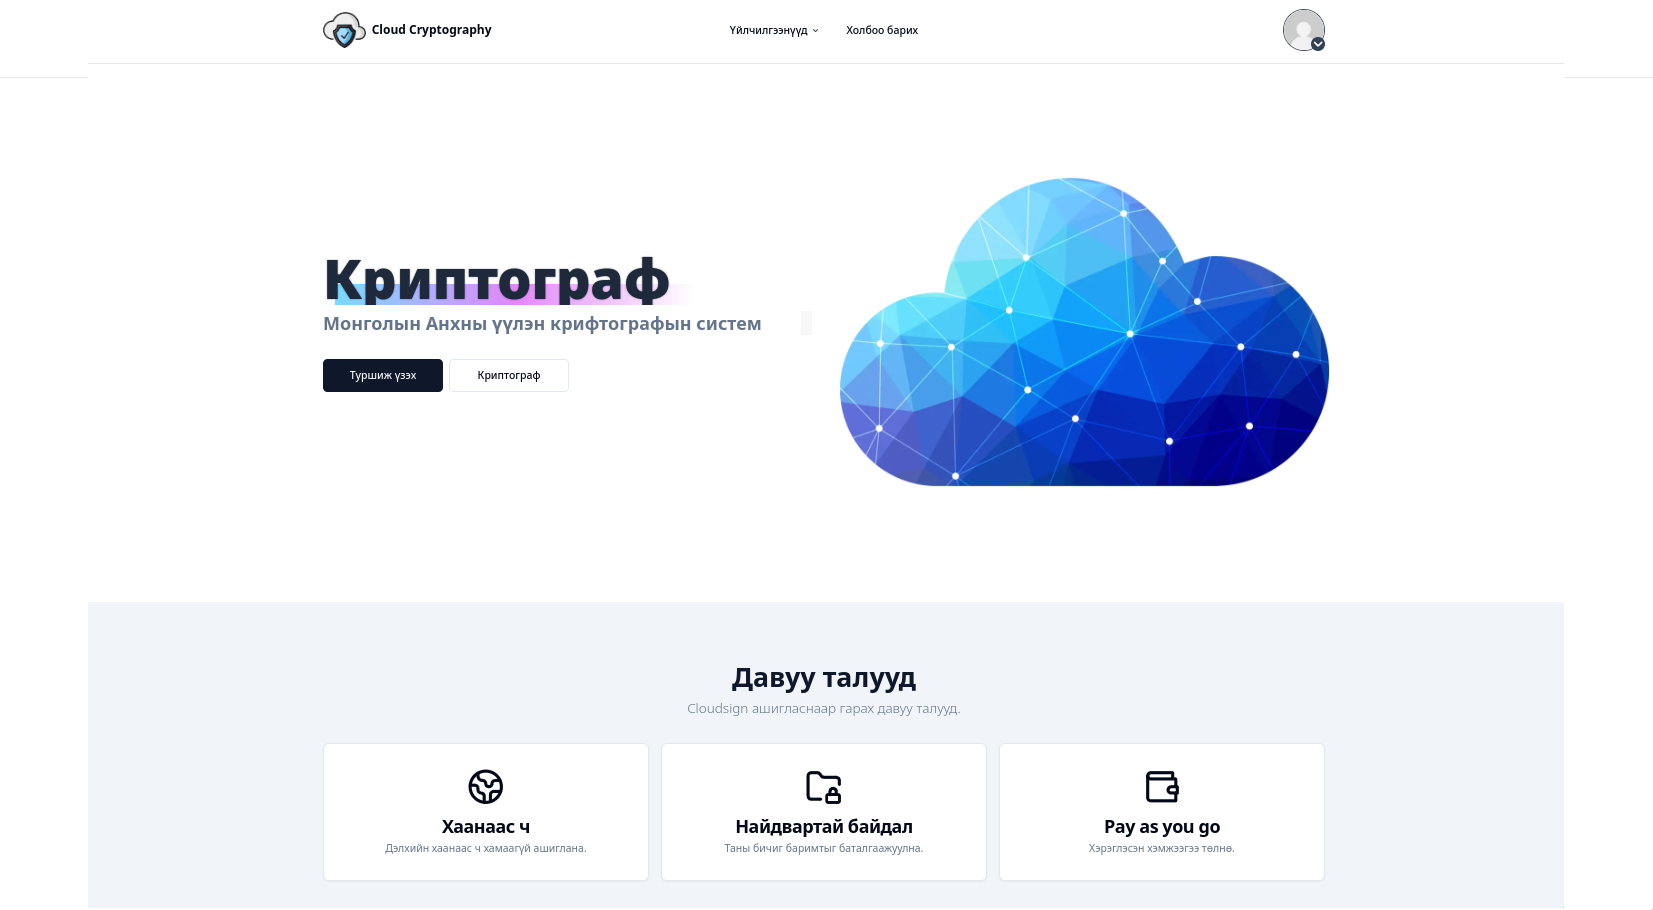
\includegraphics[scale=0.26]{assets/web/hero.png}
	\caption{Нүүр хуудас}
	\label{fig:architecture}
\end{figure}
\begin{figure}[h]
	\centering
	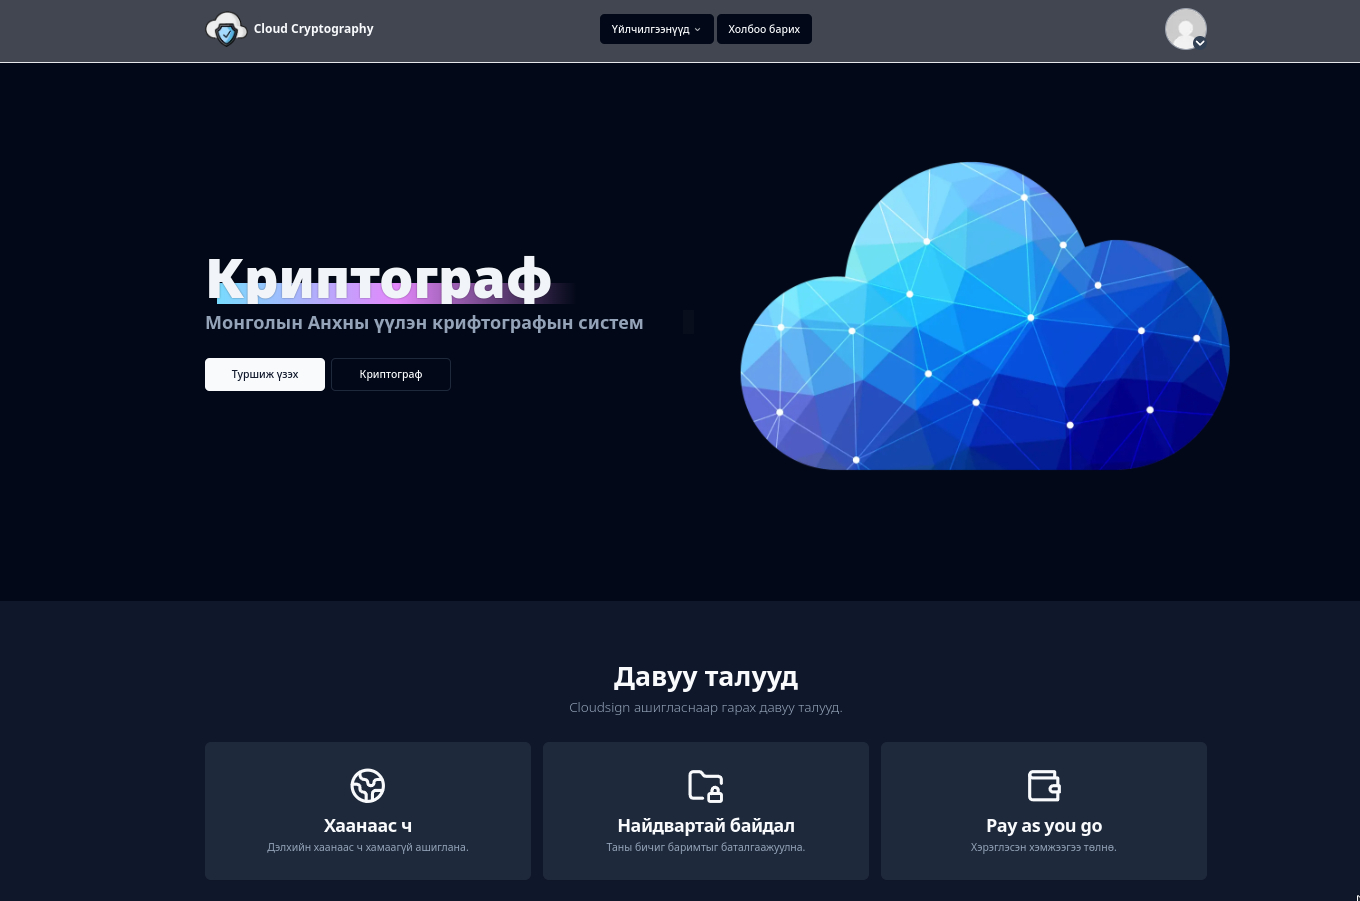
\includegraphics[scale=0.3]{assets/web/darkhero.png}
	\caption{Нүүр хуудас, Шөнийн тохиргоо}
	\label{fig:architecture}
\end{figure}
Өөрийн хувийн нийтийн түлхүүрийг, нууц үгтэйгээр үүсгэх хэсэг.
\begin{figure}[h]
	\centering
	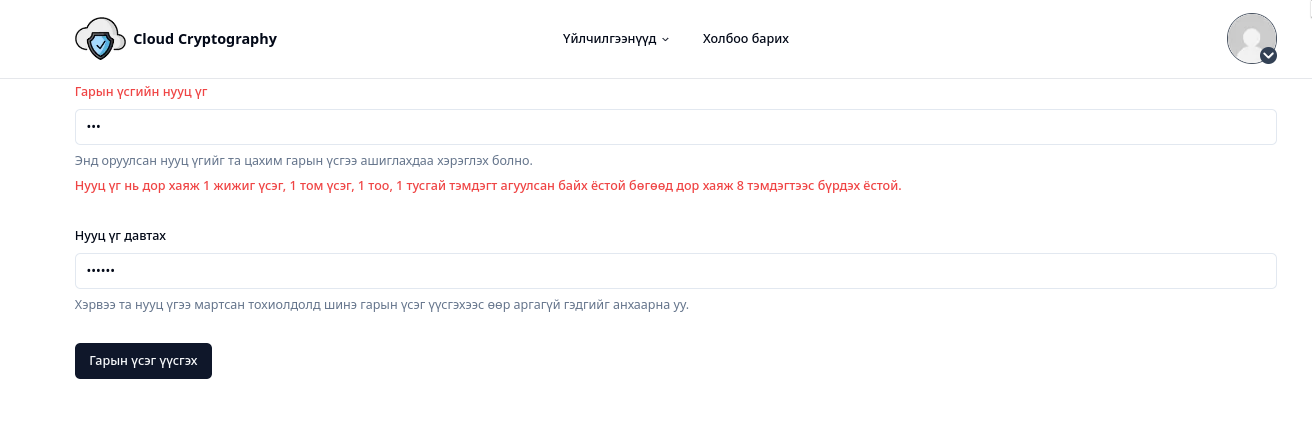
\includegraphics[scale=0.45]{assets/web/makepass.png}
	\caption{Тоон гарын үсэг үүсгэх шаардлага}
	\label{fig:architecture}
\end{figure}
\begin{figure}[h]
	\centering
	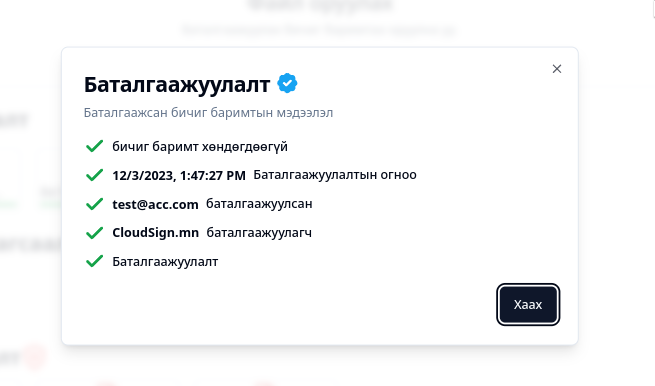
\includegraphics[scale=0.55]{assets/web/batalgaajuulaltConfirmed.png}
	\caption{Хүчинтэй гарын үсэгтэй баримт}
	\label{fig:architecture}
\end{figure}
\begin{figure}[h]
	\centering
	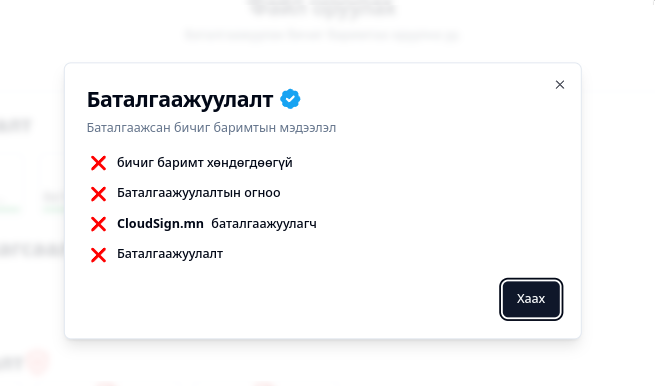
\includegraphics[scale=0.55]{assets/web/batalgaajuulaltDeclined.png}
	\caption{Хүчингүй гарын үсэгтэй баримт}
	\label{fig:architecture}
\end{figure}
\begin{figure}[h]
	\centering
	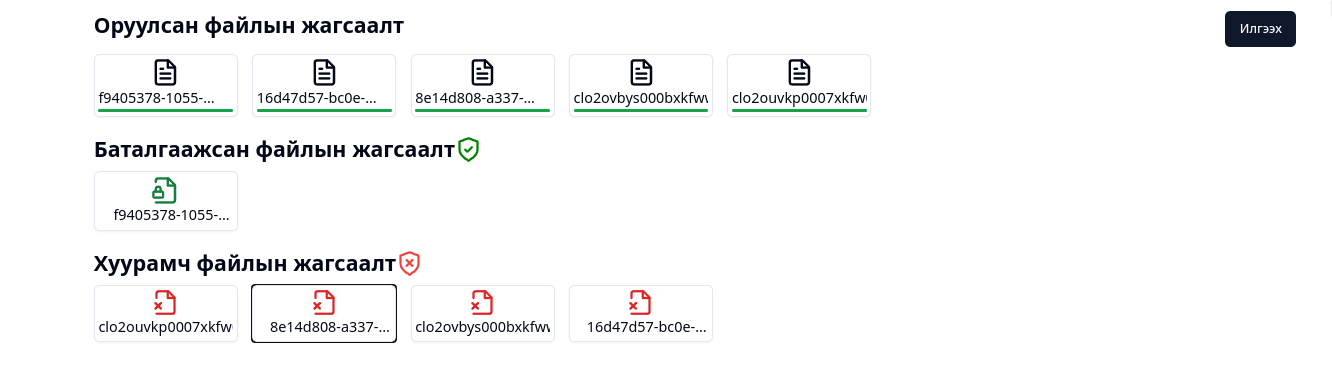
\includegraphics[scale=0.5]{assets/web/list.png}
	\caption{Нийт баримтын жагсаалт}
	\label{fig:architecture}
\end{figure}
\begin{figure}[h]
	\centering
	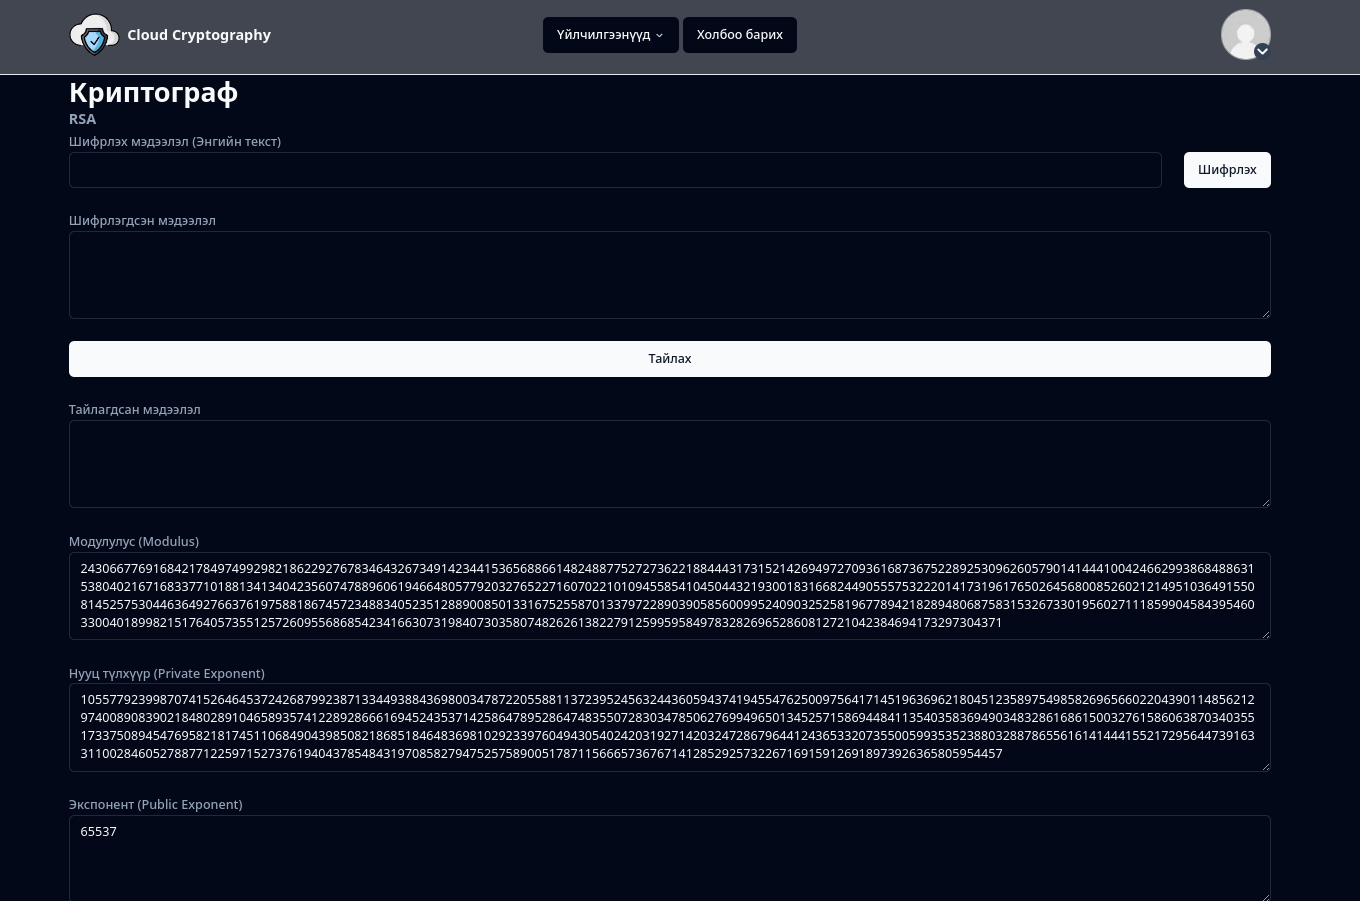
\includegraphics[scale=0.35]{assets/web/rsa.png}
	\caption{РСА (RSA) алгоритмын хэрэгжүүлэлт}
	\label{fig:architecture}
\end{figure}

\begin{figure}[h]
	\centering
	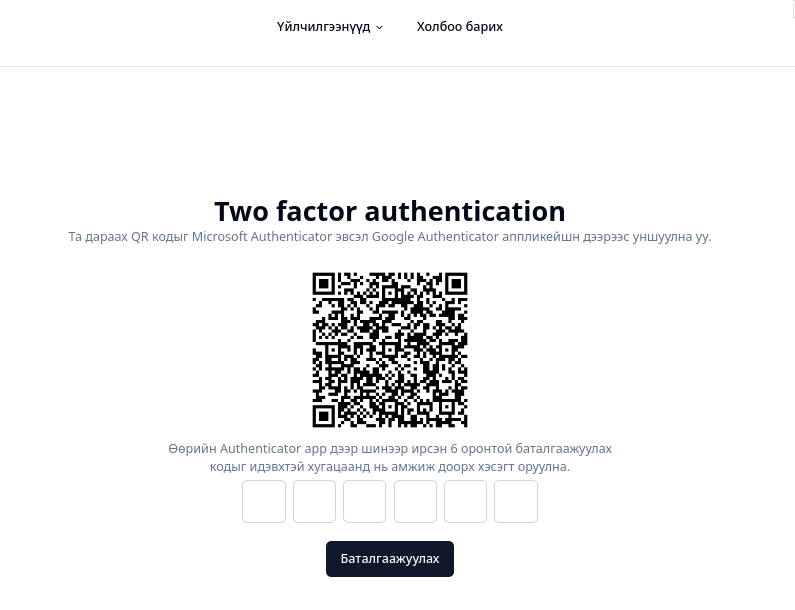
\includegraphics[scale=0.55]{assets/web/2fa.png}
	\caption{Цагаас хамаарсан нууц үг тохируулах}
	\label{fig:architecture}
\end{figure}
\begin{figure}[h]
	\centering
	
\includegraphics[scale=0.65]{assets/web/2faconfirm.png}
	\caption{Цагаас хамаарсан нууц үг тохируулсны дараа}
	\label{fig:architecture}
\end{figure}